\documentclass[17pt]{beamer}
%\documentclass[aspectratio=169,17pt]{beamer}
\usepackage{fontspec}
\defaultfontfeatures{Mapping=tex-text}

\mode<presentation>
\usetheme[height=1.5\baselineskip]{Waterloo}

%%%%%%%%%%%%%
%% OPTIONS %%
%%%%%%%%%%%%%

% make whale theme super striking
\setbeamercolor*{frametitle}{parent=palette primary}

% make whale theme more subtle
%\setbeamercolor*{block title}{use=structure,fg=black,bg=structure.fg}

% by default dark titles; change to light with
%\usecolortheme{seahorse}
%\usecolortheme{rose}

% navigation symbols are lame; get rid with
\setbeamertemplate{navigation symbols}{}

% use serifs for math (kind of necessary)
\usefonttheme[onlymath]{serif}

%%%%%%%%%%%%%%%%%%%%%%%%%%
%% NO MORE REAL OPTIONS %%
%%%%%%%%%%%%%%%%%%%%%%%%%%

\usepackage{graphicx}
\usepackage{textcomp}
\setsansfont{Lato}
\setmonofont{Inconsolata}

% Center a figure
\newcommand{\cf}[2]{
    \begin{center}
      \includegraphics[width=#2\columnwidth]{#1}
    \end{center}
  }

\graphicspath{{figures/}}

%%%%%%%%%%%%%%%%%%%%%%%
%% PRESENTATION INFO %%
%%%%%%%%%%%%%%%%%%%%%%%

\title{Open Data in Neuroscience}
\author{Trevor Bekolay}
\institute{University of Waterloo}
\date{April 6, 2013}

%%%%%%%%%%%%%%%%%%
%% PRESENTATION %%
%%%%%%%%%%%%%%%%%%

\setbeamercovered{transparent=0}

\begin{document}

\frame[plain]{\titlepage}

\begin{frame}[plain]
  %% \vspace{-pt}
  \cf{spaun}{0.73}
\end{frame}

\begin{frame}[plain]
  %% \vspace{-20pt}
  \hspace*{-.04\columnwidth}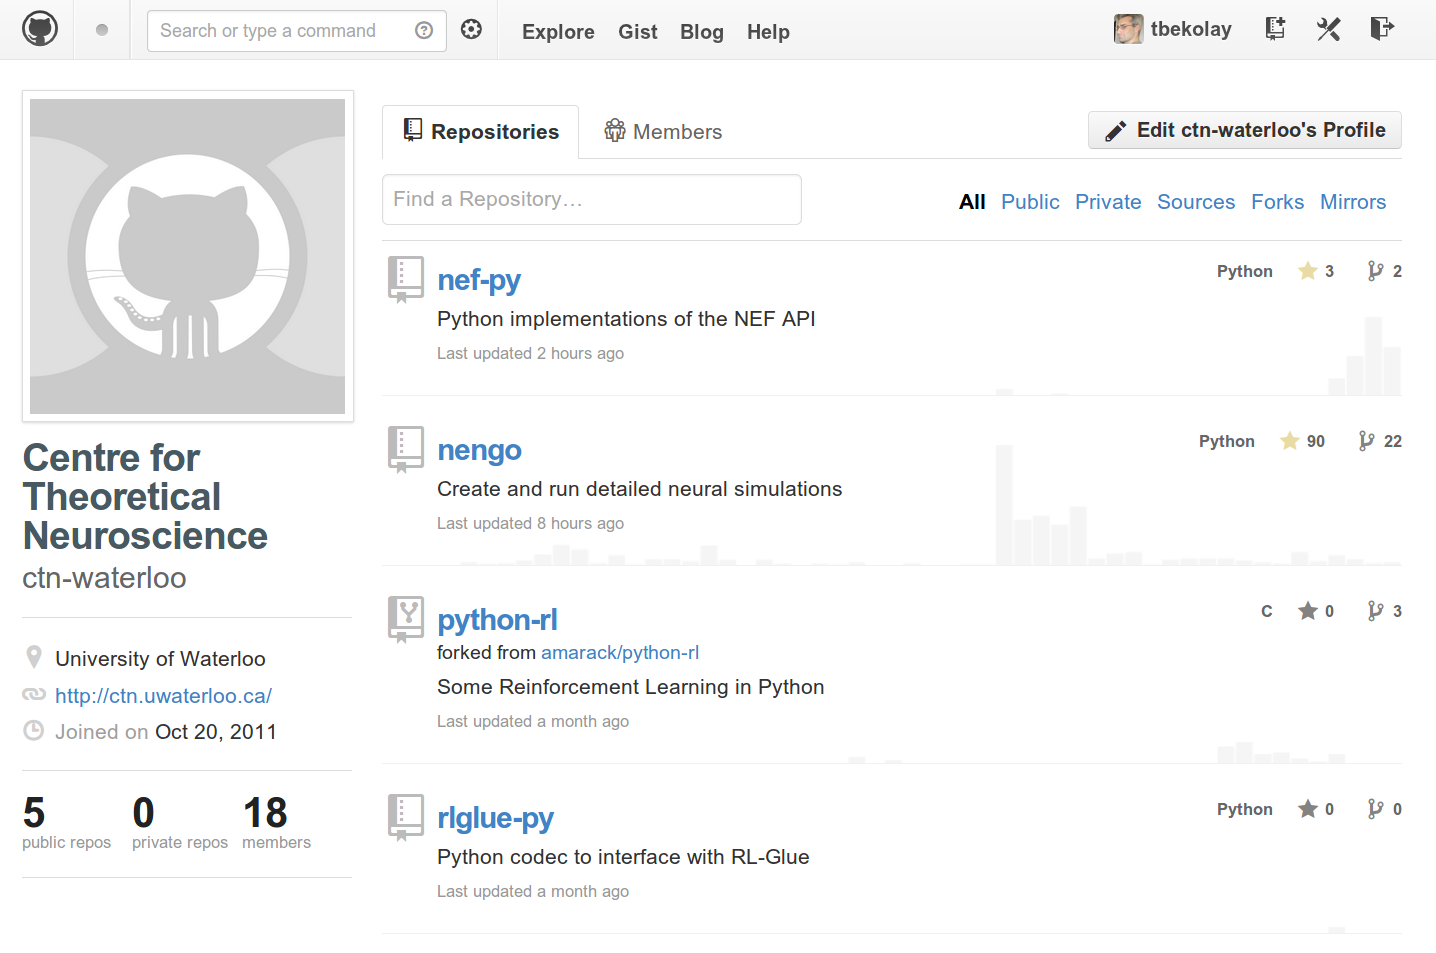
\includegraphics[width=1.09\columnwidth]{github}
\end{frame}

\begin{frame}[plain]
  \begin{center}
    \begin{huge}
      \textbf{1. Precious data}
    \end{huge}
  \end{center}
\end{frame}

\begin{frame}[plain]
  \begin{center}
    \begin{huge}
      \textbf{2. Closed culture}
    \end{huge}
  \end{center}
\end{frame}

\begin{frame}[plain]
  \begin{center}
    \begin{huge}
      \textbf{3. How?}
    \end{huge}
  \end{center}
\end{frame}

\begin{frame}[plain]
  \vspace{-40pt}
  \begin{center}
    \begin{huge}\textbf{3. How?}\end{huge}
  \end{center}
  \vspace{1em}
  \begin{columns}
    \begin{column}{0.3\textwidth}
      \cf{figshare}{1.0}
    \end{column}
    \begin{column}{0.35\textwidth}
      \cf{datadryad}{1.0}
    \end{column}
    \begin{column}{0.25\textwidth}
      \cf{datahub}{1.0}
    \end{column}
  \end{columns}
\end{frame}

\begin{frame}[plain]
  \vspace{-12pt}
  \begin{center}
    \begin{huge}\textbf{2. Closed culture}\end{huge}
  \end{center}
  \vspace{0.5em}
  \begin{center}
    
\includegraphics[width=0.8\columnwidth]{nif} \\ \vspace{1em}
    
\includegraphics[width=0.8\columnwidth]{neurotycho}
  \end{center}
\end{frame}

\begin{frame}[plain]
  \vspace{-16pt}
  \begin{center}
    \begin{huge}\textbf{1. Precious data}\end{huge}
  \end{center}
  \vspace{0.5em}
  \begin{center}
    
\includegraphics[width=0.8\columnwidth]{neurosynth} \\ \vspace{1em}
    
\includegraphics[width=0.8\columnwidth]{neuroelectro}
  \end{center}
\end{frame}

\begin{frame}[plain]
  \begin{center}
    \begin{Large}
      Slides and URLs at \\ \vspace{0.6em}
      \url{github.com/tbekolay/odx13}
    \end{Large}
  \end{center}
\end{frame}

\end{document}

